\section{Data link layer}
The data link layer is implemented as a DataLinkLayer class and a Frame class.
The DataLinkLayer object is instantiated by the backbone class and controls the
network token and the processing of frames into datagrams and vice versa. When
instantiating, the address and token is controlled by arguments. The Frame
objects and datagram objects are instantiated in buffers by the backbone and
presented to the data link layer as method arguments.

\begin{figure}[htb]
	\begin{center}
	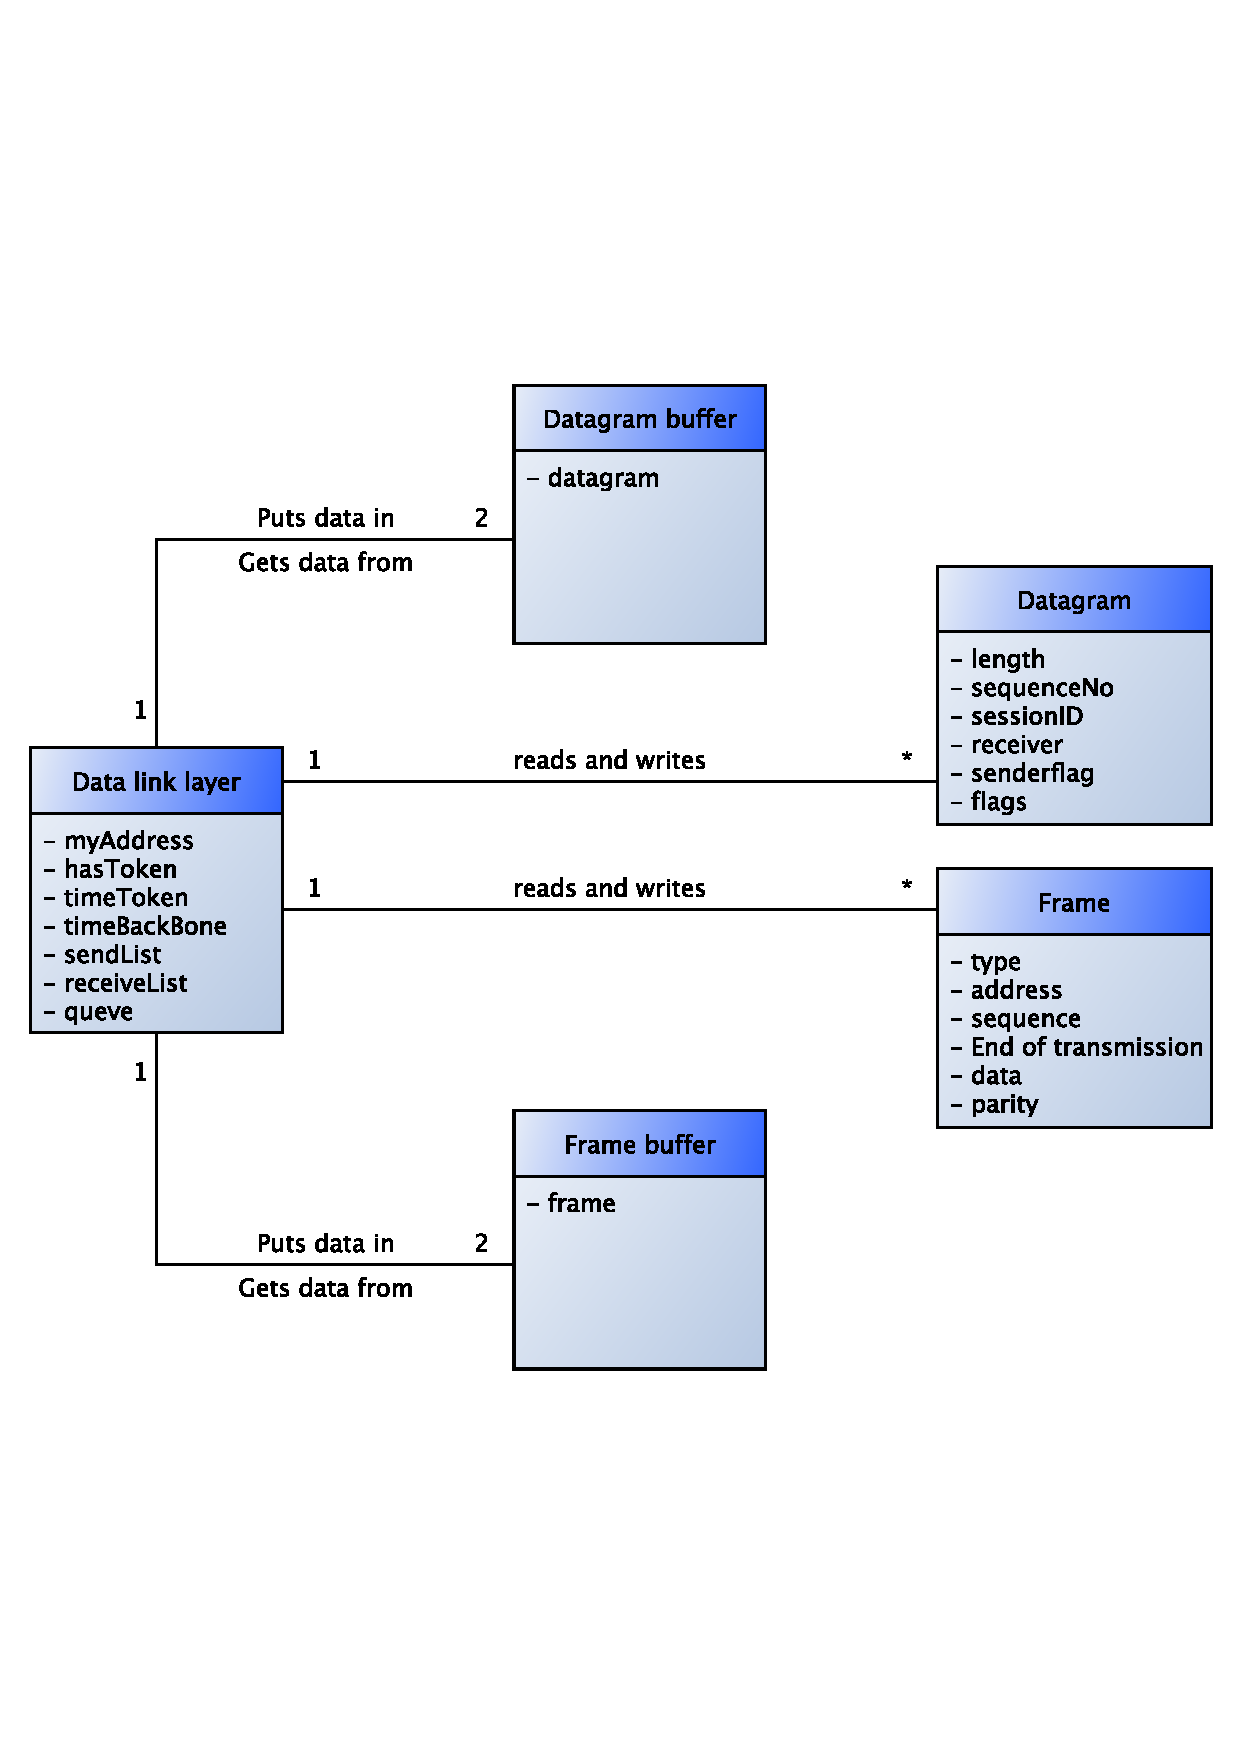
\includegraphics[scale=0.5,trim=0 170 0 170]{dll_domainmodel.pdf}
	\caption{Domain model for data link layer}
	\label{fig:class_diag_for_datalink}	
	\end{center}
\end{figure}

Two public methods are used to call the data link layer, one for upwards traffic
(decode) and one for downwards traffic (encode). Both methods are called with
pointers to the four accessible buffers as arguments. Furthermore the backbone
can call a method (needsAttention) to know whether the data link layer need
extraordinary attention because a timer has run out. Another method
(canTransmit) telles the backbone whether the data link layer object holds the
network token and thereby is able to send encoded data.

\begin{figure}[htb]
	\begin{center}
	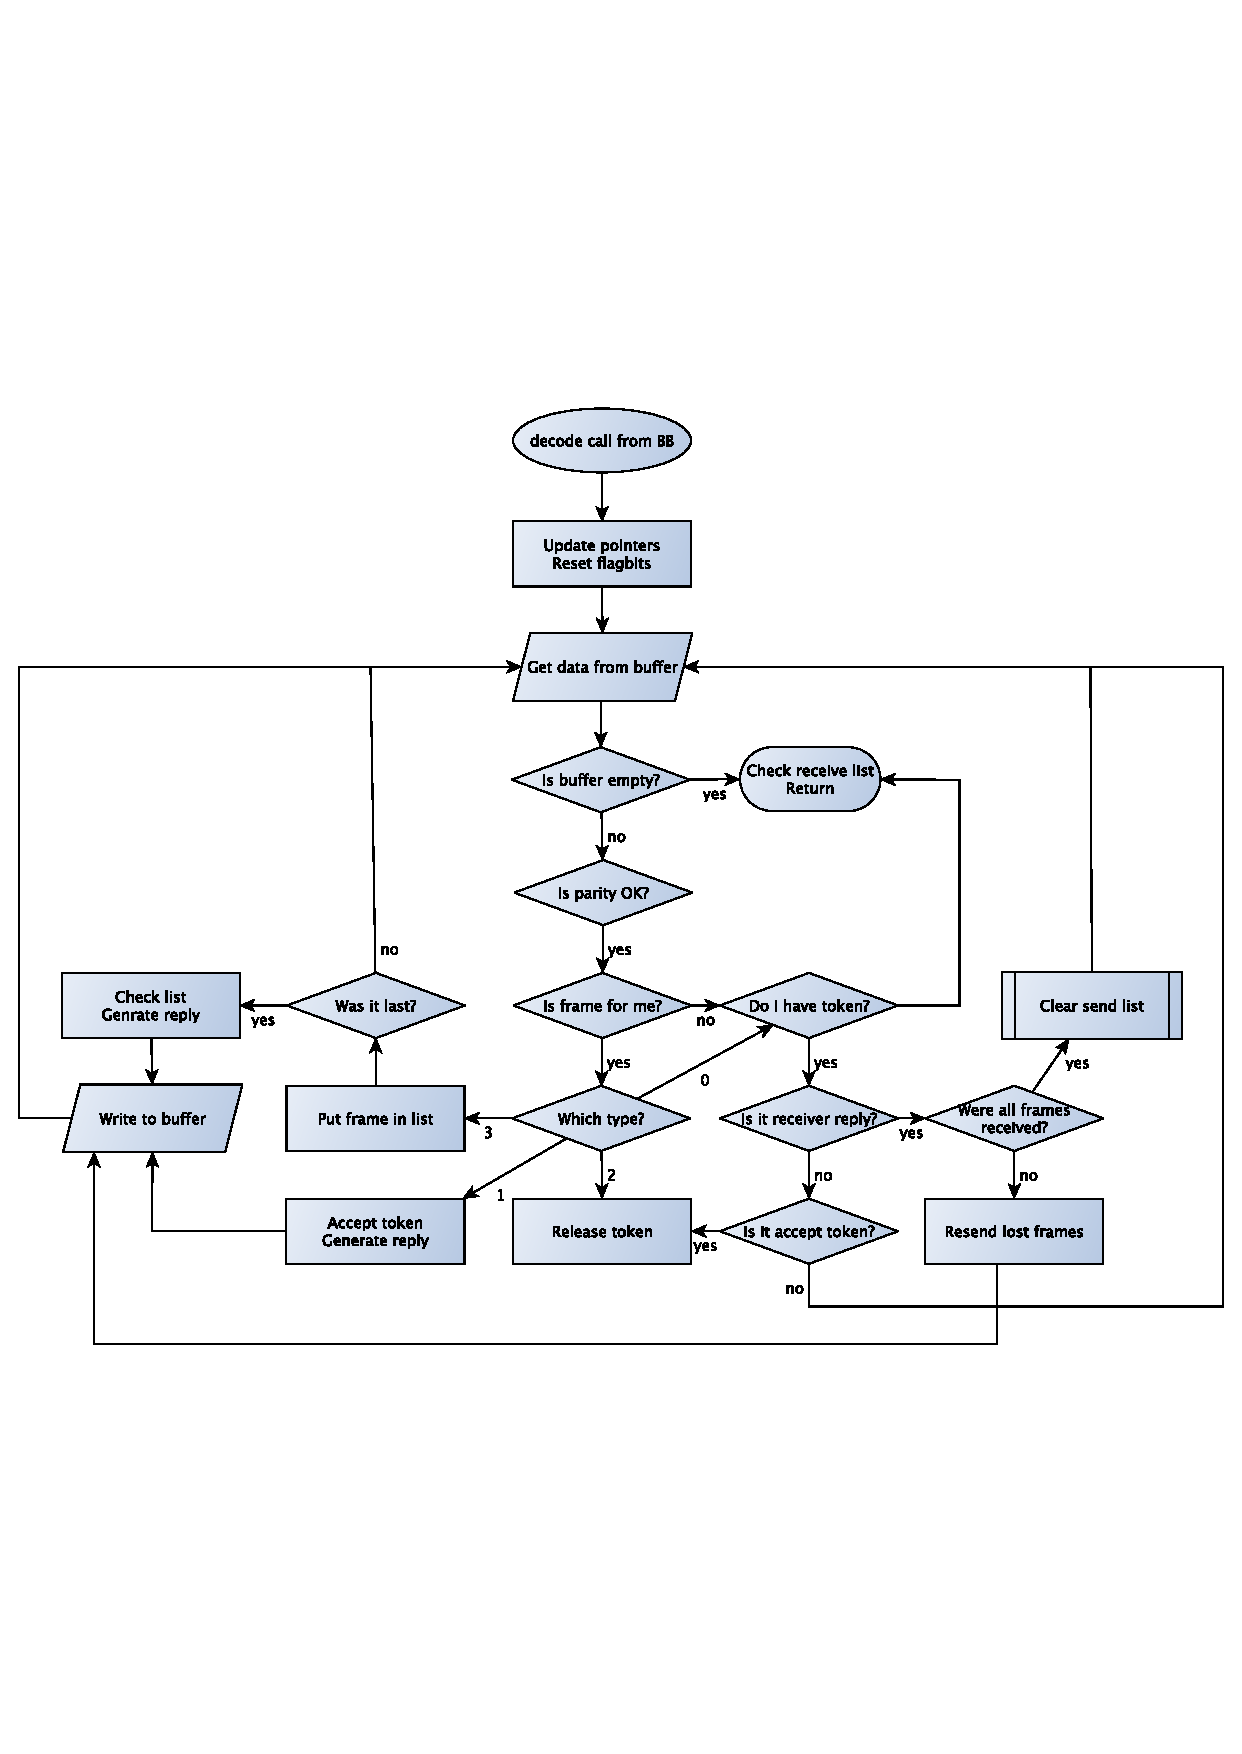
\includegraphics[scale=0.5,trim=0 190 0 190]{dll_flow_decode.pdf}
	\caption{Flow chart for data link layer decode method}
	\label{fig:dll_flow_decode}	
	\end{center}
\end{figure}

The methods of the classes are developed to realize the flowchart of the data
link layer. Decisions on whether to implement a method in one class or another
is done using the expert pattern.

\begin{figure}[htb]
	\begin{center}
	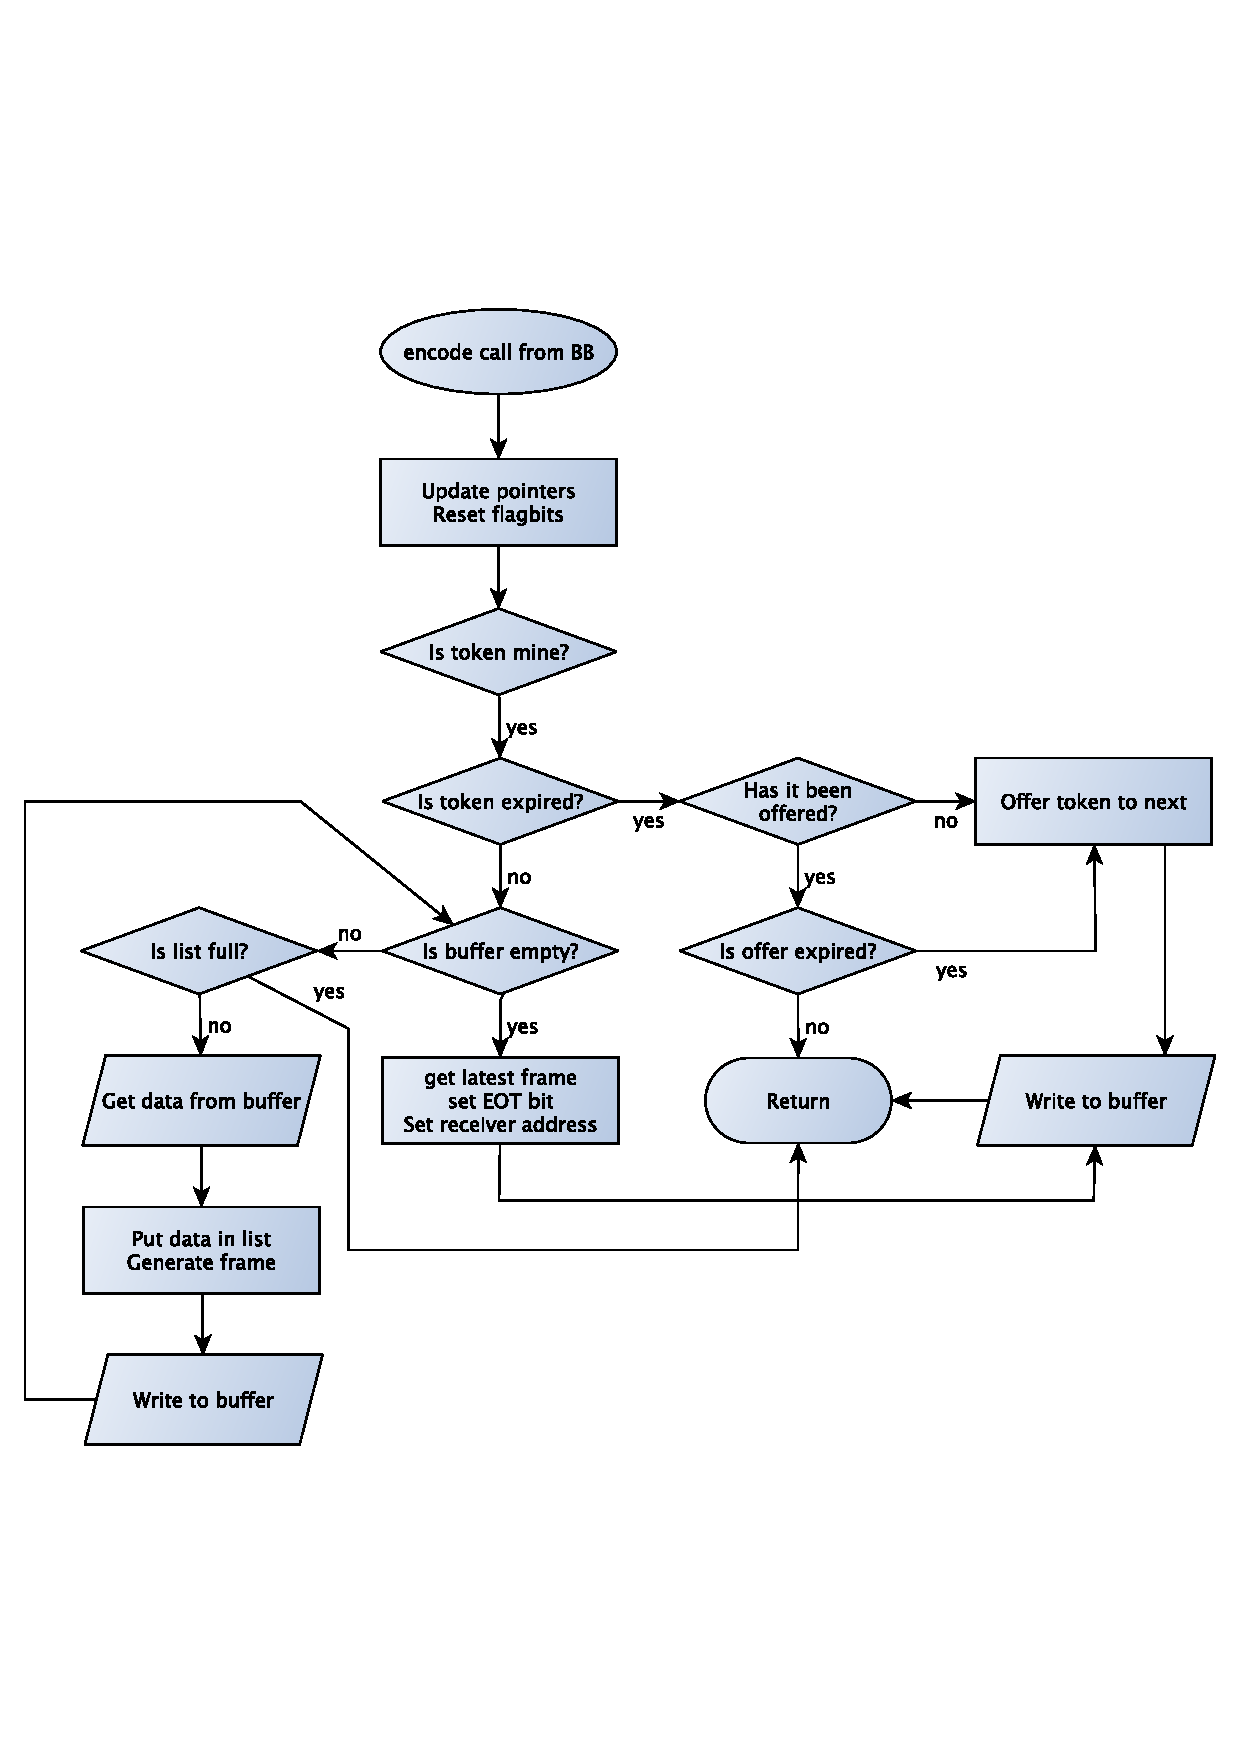
\includegraphics[scale=0.5,trim=0 140 0 140]{dll_flow_encode.pdf}
	\caption{Flow chart for data link layer encode method}
	\label{fig:dll_flow_encode}	
	\end{center}
\end{figure}
